\newpage
\section{Kamera}
Det indkøbte kamera viste ikke at have tilstrækkelig kvalitet igennem en enhedstest. Der kunne ikke skelnes mellem det eksokrine væv og de langerhanske øer. Yderligere blev det erfaret, at lyset er utrolig vigtigt, derfor er ideen med kamerahuset en nødvendighed for at kontrollere lyset til kameraet. Der kan læses mere om enhedstesten af kameraet i afsnit 4.3.1 \fxnote{Tjek ref} i projektdokumentationen. Til at erstatte kameraet blev der i stedet genereret en række billeder, som skulle simulere flowet af opløsningsvæske igennem slangen.

\subsection{Kamerasimulation}
Til at generere et billedsæt, der simulerer langerhanske øer, er der udviklet et Matlab script. Billederne, der er valgt, stammer fra det indkøbte kamera. Grunden til de kan anvendes som grundlag for genereringen af billeder, på trods af kameraets utilstrækkelige kvalitet, er, at øerne og det ekstra væv er adskilt i de enkelte billeder. Dette muliggør en separat segmentering af øer og væv, som herefter kan sammensættes til billeder, der ligger tæt op af det der observeres gennem et almindeligt mikroskop. De 3 billeder, der danner grundlag for billedgenereringen, er vist nedenfor. 
\begin{figure}[H] \centering
\begin{minipage}[b]{0.3\textwidth} \centering
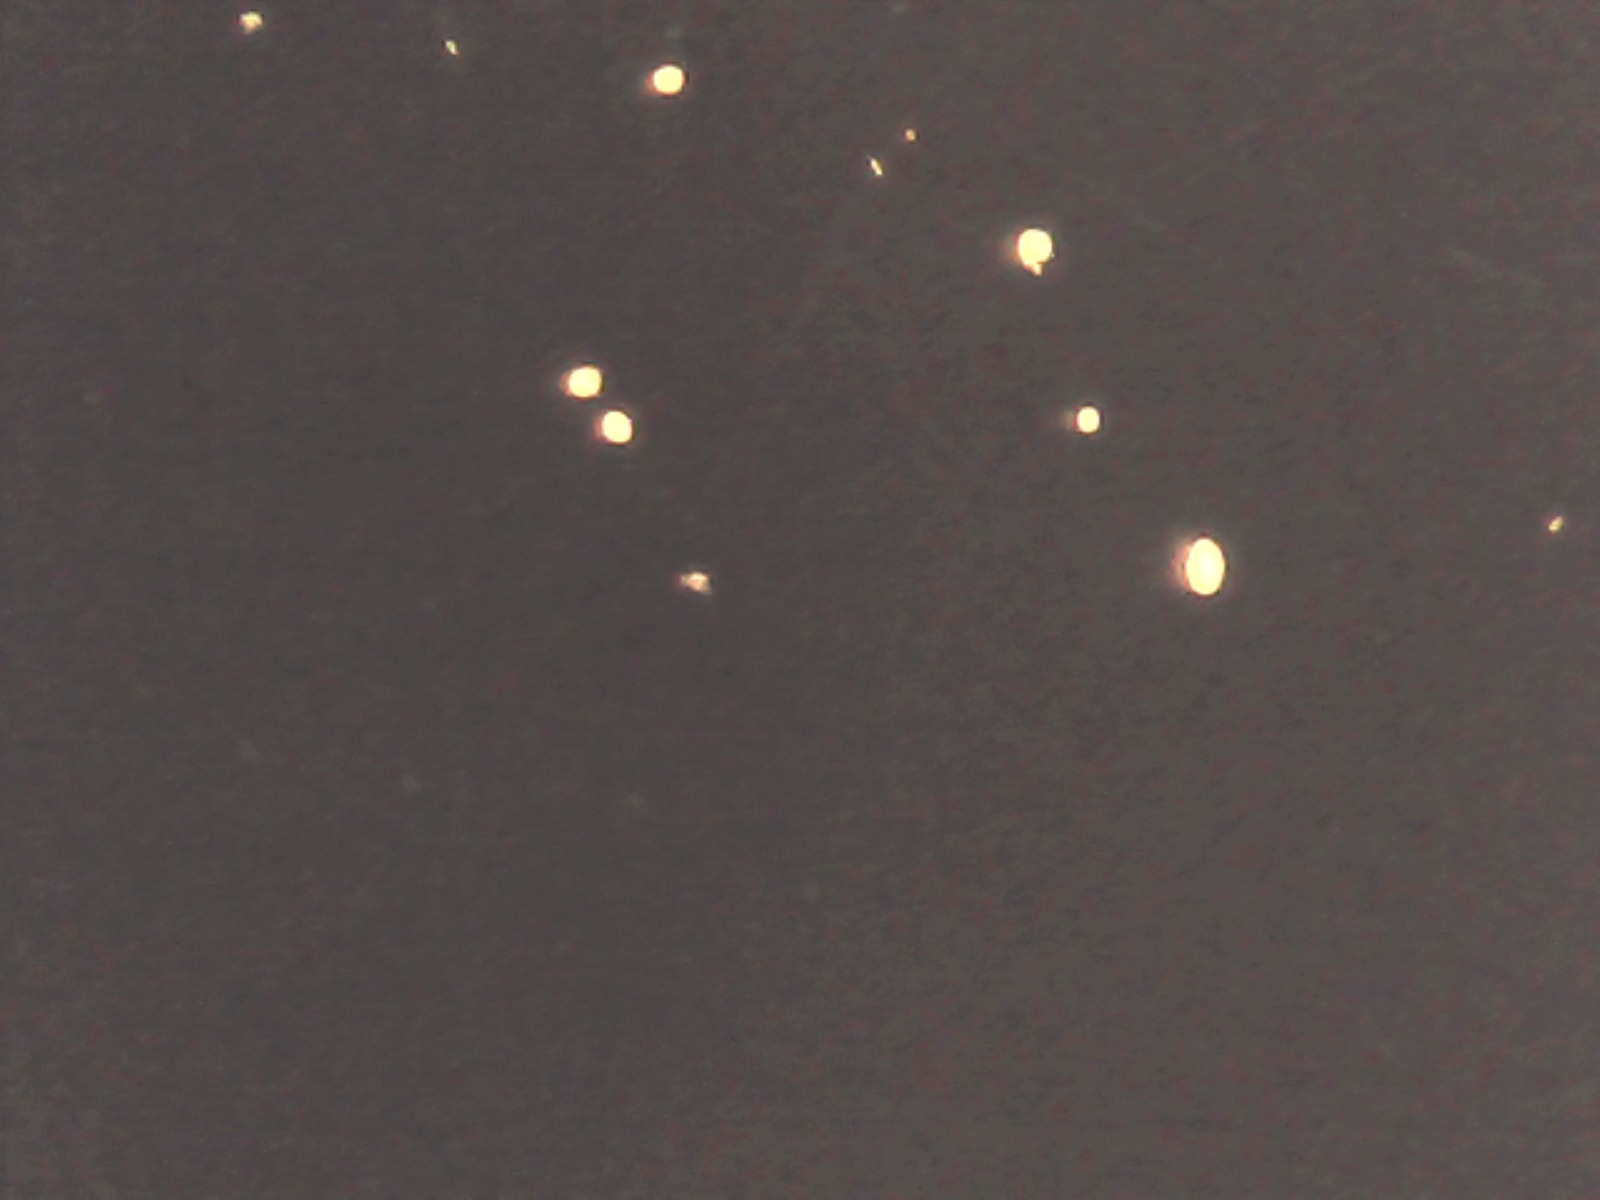
\includegraphics[width=1.00\textwidth]{billeder/software/1.jpg} % Left picture
\end{minipage} \hfill
\begin{minipage}[b]{0.3\textwidth} \centering
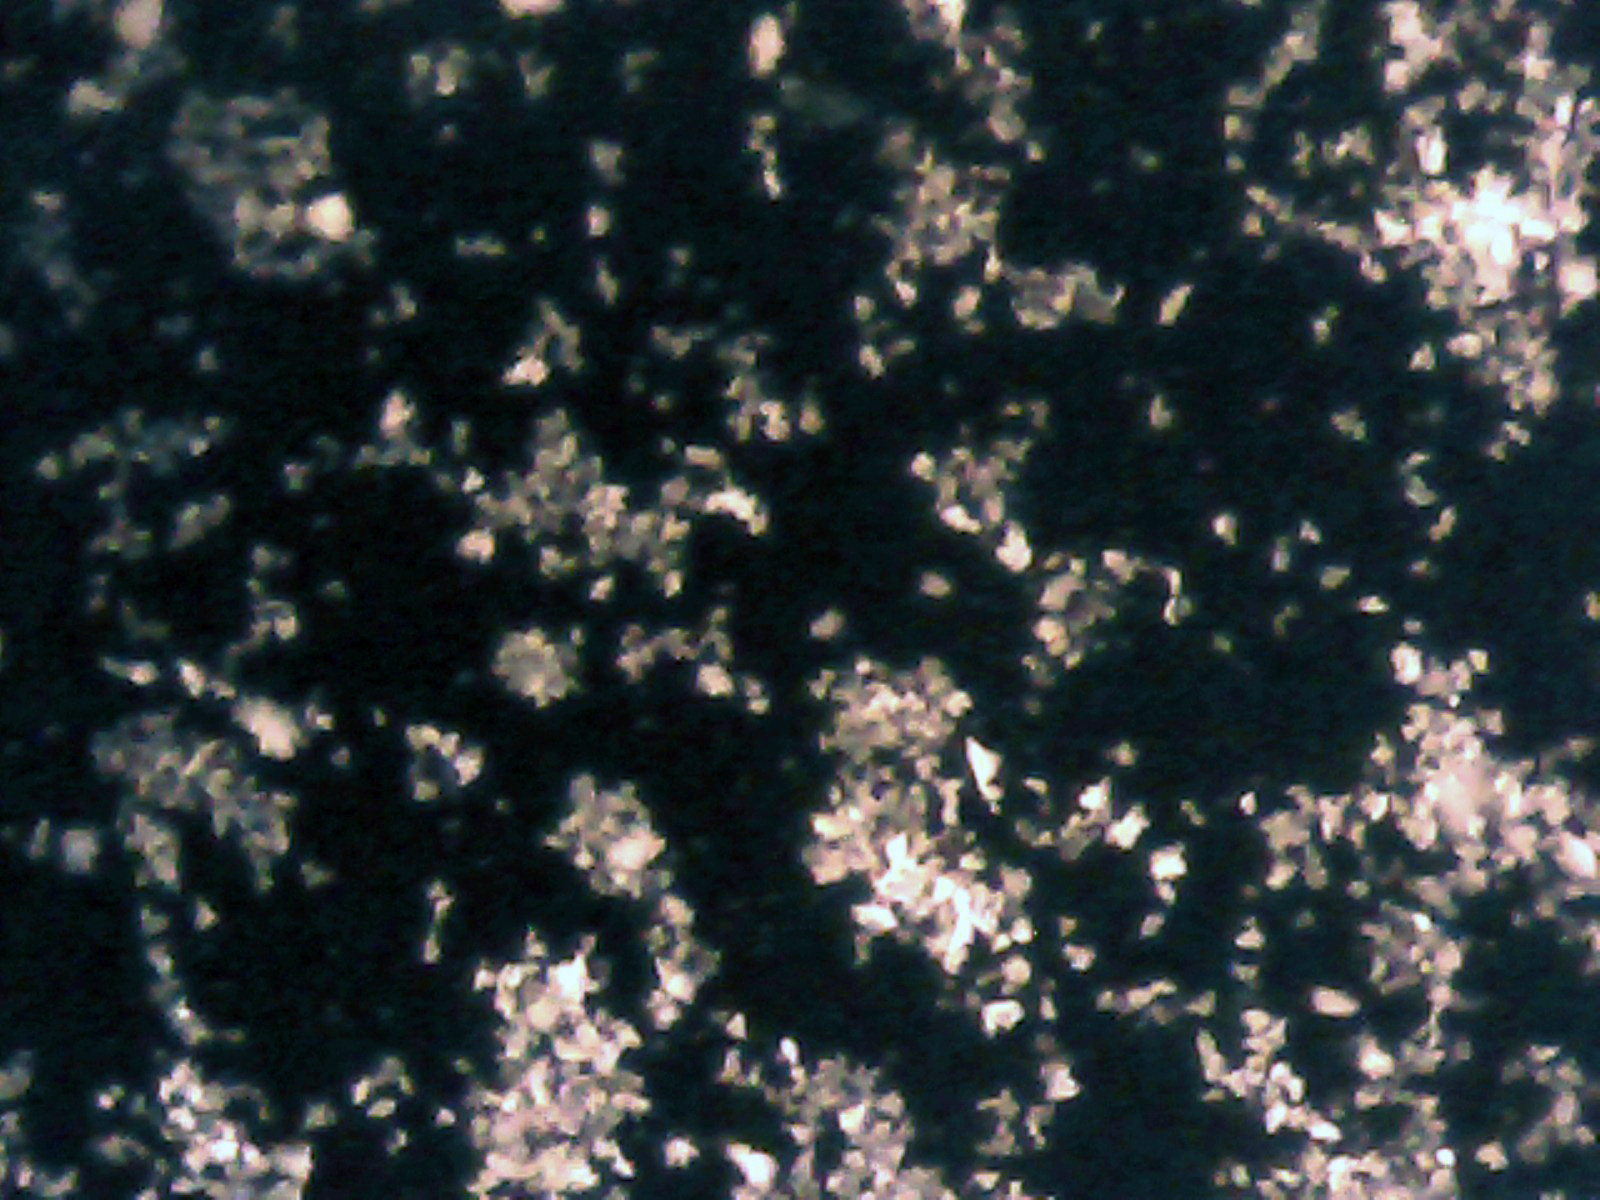
\includegraphics[width=1.00\textwidth]{billeder/software/2.jpg} % Right picture
\end{minipage} 
\hfill
\begin{minipage}[b]{0.3\textwidth} \centering

\includegraphics[width=1.00\textwidth]{billeder/software/3.jpg} % Right picture
\end{minipage} \\  % Captions og labels
\begin{minipage}[t]{0.3\textwidth}
\caption{Billede indehold-ende langerhanske øer} % Left caption and label
\label{fig:img1}
\end{minipage} \hfill
\begin{minipage}[t]{0.3\textwidth}
\caption{Billede inde-holdende ekstra væv} % Right caption and label
\label{fig:img2}
\end{minipage}
\hfill
\begin{minipage}[t]{0.3\textwidth}
\caption{Baggrundsbillede} % Right caption and label
\label{fig:img3}
\end{minipage}
\end{figure}
Flowsimuleringen er opbygget på en måde, hvor den består af henholdsvis en sekvens indeholdende en langerhansk ø efterfulgt af en sekvens uden en ø. I selve programmet indlæses et nyt billede hvert 0,1 sekund. Derfor skal der generes en passende mængde billeder, som programmet kan indlæse. Simuleringen er implementeret, så der minimum genereres 252 eller maksimalt 432 billeder, hvilket giver en samlet sekvenslængde på 25,2 sekunder eller 43,2 sekunder. Grunden til, at antallet af billeder varierer, er, at længden af sekvensen uden en langerhansk ø bestemmes udfra en random variabel. Dette gøres for at simulere, at der kan være variabel tid mellem en ny ø kommer igennem slangen. I scriptet genereres der i alt 18 fulde sekvenser. Det betyder, at der passerer imellem 25 og 43 øer i minuttet. Antallet af øer, der passere pr. minut, er bestemt ud fra formel \ref{formular:isletprmin}: 
\begin{align}
\frac{18\text{ sekvenser}}{\frac{n}{10}} * 60s = \text{Antal øer pr. minut}
\text{ , hvor n er antallet af billeder i sættet}
\label{formular:isletprmin}
\end{align} 
I figur \ref{fig:boxplot} er vist et boxplot, som viser distributionen af hvor mange øer der passerer i minuttet. Det ses at medianen ligger over 30 øer pr. minut, hvilket betyder, at der i gennemsnit vil blive sorteret over 30 øer pr minut. De 30 øer pr. minut stammer fra hastighedskravet fra systemets kvalitetskrav (Se kravspecifikationen i projektdokumentationen)

 \begin{figure}[H]
	\centering
	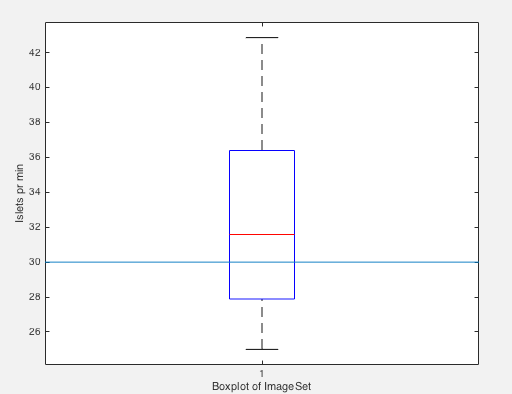
\includegraphics[width=0.5\textwidth]{billeder/software/boxplot.png}
	\caption{Boxplot af distrubutionen af øer pr. minut}
	\label{fig:boxplot}
\end{figure}

Selve flowsimuleringen sker i et for loop, hvor positionen for øen flyttes for hver iteration. I figur \ref{fig:flowsim} er flow simulationen illustreret for de i alt 18 sekvenser, med en graf for hver ø. Det ses at øen flytter sin Y position tilfældigt, mens X positionen springer med et fast interval for hver iteration i for loopet.

\begin{figure}[H]
	\centering
	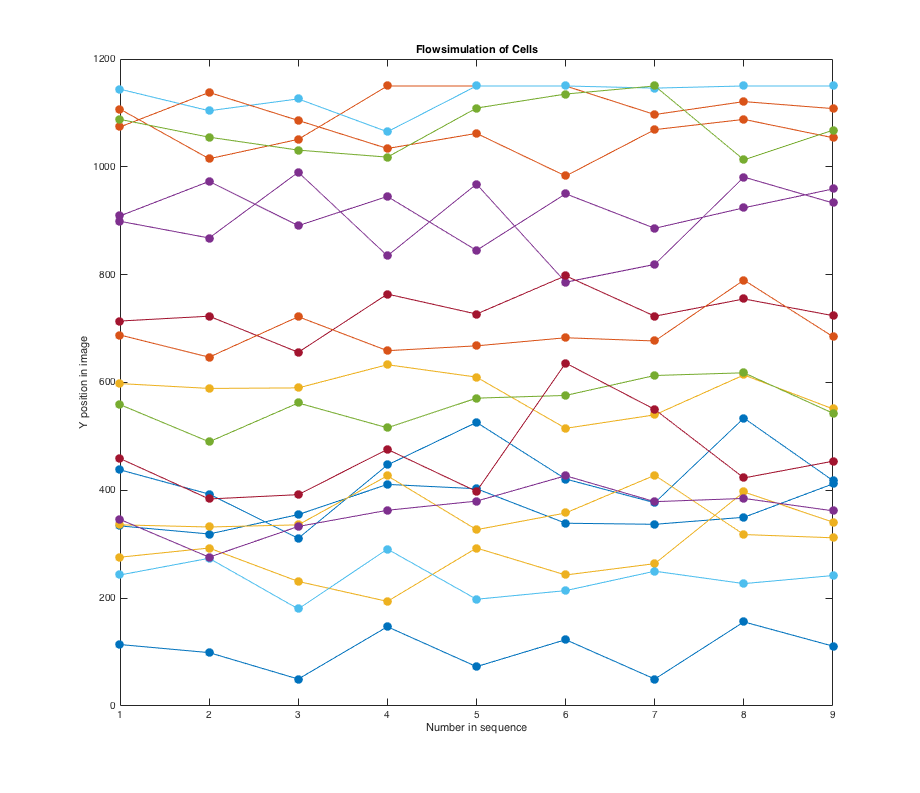
\includegraphics[width=0.5\textwidth]{billeder/software/Simulation.png}
	\caption{Illustration over flow simuleringen}
	\label{fig:flowsim}
\end{figure}


Øens position på billedet ændres ved en normalfordelt random variabel med mean på 0 og standard afvigelse(sd) på 50 pixels. Nedenstående figur \ref{fig:histfit} viser fordelingen af pixels øen flyttes for hver iteration. På figur \ref{fig:histfit} er der vist markører for standard afvigelsen ($\sigma$) og $2*$standard afvigelsen ($2\sigma$) for hver side af mean. Imellem $-\sigma$ og $\sigma$ er der 68,26 \% sandsynlighed for, at den nye Y position ville ligge inden for dette område. For 2 sd afvigelse ($2\sigma$) er der 95,45 \% for, at den nye Y position vil ligge indenfor dette område.

\begin{figure}[H]
	\centering
	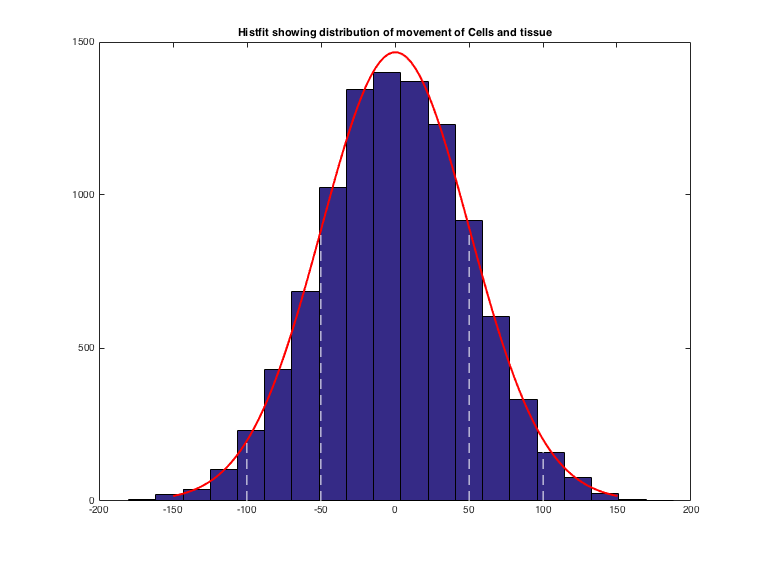
\includegraphics[width=0.5\textwidth]{billeder/software/histfit.png}
	\caption{Histogram over fordelingen af ny Y position}
	\label{fig:histfit}
\end{figure}

Det endelige resultat af billedegeneringen er vist i figur \ref{fig:finalresult}. Til at illustrere hvordan øen flytter sig er der tilføjet en graf, som viser hvordan dens position ændres for hver iteration. Øen er markeret med en rød ring på billedet.

\begin{figure}[H]
	\centering
	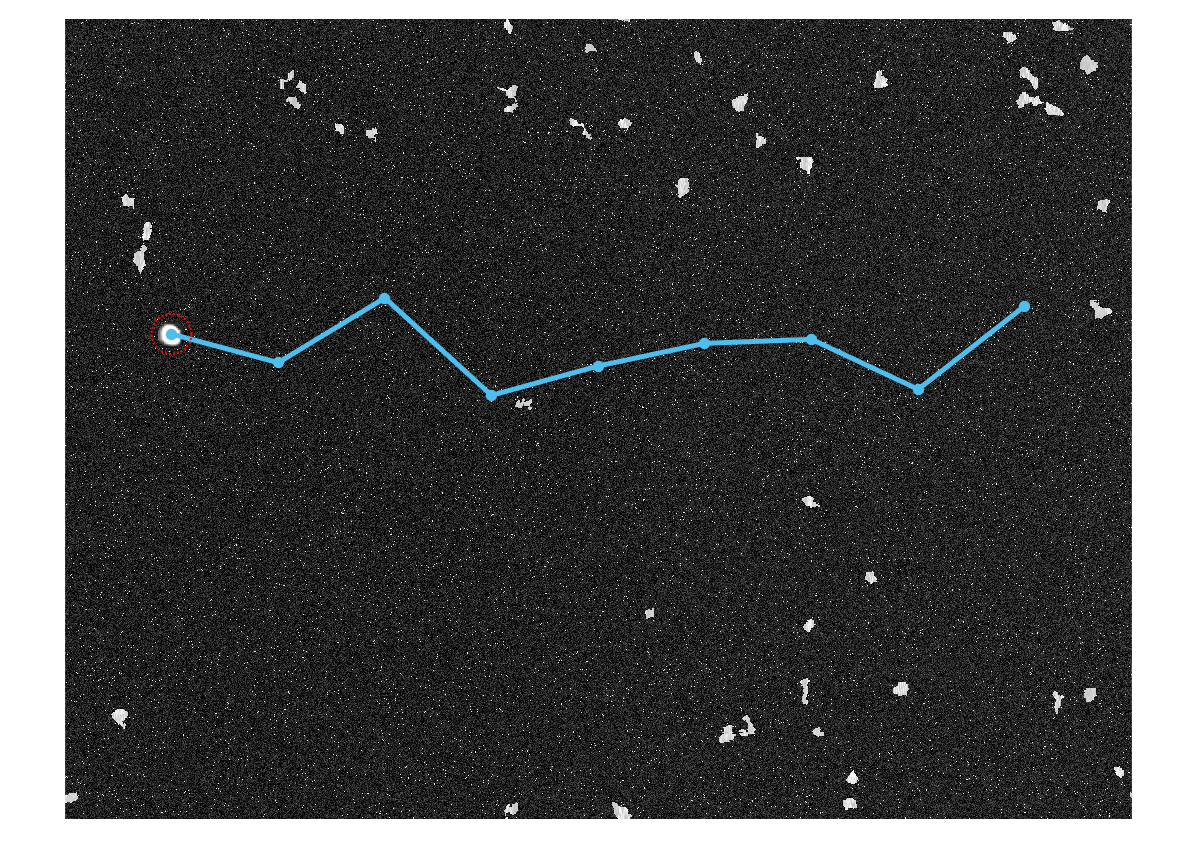
\includegraphics[width=0.7\textwidth]{billeder/software/final.png}
	\caption{Endelige resultat for flowsimulering}
	\label{fig:finalresult}
\end{figure}

\newpage
\subsection{Billedprocessering}
Segmenteringen sker via en række morfologiske operationer, hvor billedet fra kamera simulationen konverteres til en logisk maske. Detektionenen baseres på, at øerne har en mere cirkulær form end resten af vævet. Derfor hentes der egenskaber fra objekterne i masken vha. \textit{Matlab} funktionen \textit{regionsprops}. De egenskaber, der hentes, er med til at beskrive hvor cirkulært objektet er. Egenskaberne er; arealet, centerpositionen, omkredsen og excentriciteten. Excentriciteten beskriver hvor langstrakt objektet er. Hvis excentriciteten er 0 er det en perfekt cirkel mens det vil være en langstrakt ellipse hvis værdien er 1.

Ud fra arealet og omkredsen af objekterne anvendes de 2 nedenstående formler til bestemmelse af 2 værdier for radiusen af objektet:
\begin{align}
Areal = R1^2*\pi => R1 = \sqrt{\frac{\text{Areal}}{\pi}}
\end{align}
\begin{align}
Omkreds = 2*R2*\pi => R2 = \frac{\text{Omkreds}}{2*\pi}
\end{align}

Ud fra disse 2 radius værdier, vil det objekt, hvor der er mindst forskel imellem de 2, være det objekt der er mest cirkulært. Til at illustrere dette er der i figur \ref{fig:circleelip} vist en cirkel og en ellipse, begge med samme areal. Ud fra \textit{regionsprops} og de 2 formler for radius kan der bestemmes 2 radiuser for henholdsvis cirklen og ellipsen. Forskellen bestemmes ved at trække de 2 beregnede værdier fra hinanden. I udregningerne nedenfor er den første kolonne værdier for cirklen, mens den anden er for ellipsen. Som det ses, er forskellen mindst ved cirklen, hvilket indikerer, at den er mest cirkulær.
  
\begin{lstlisting} 
r1 =  100.0017   99.9380

r2 =  99.7978  105.7890

rDif = 0.2039    5.8510
\end{lstlisting} 

\begin{figure}[H]
	\centering
	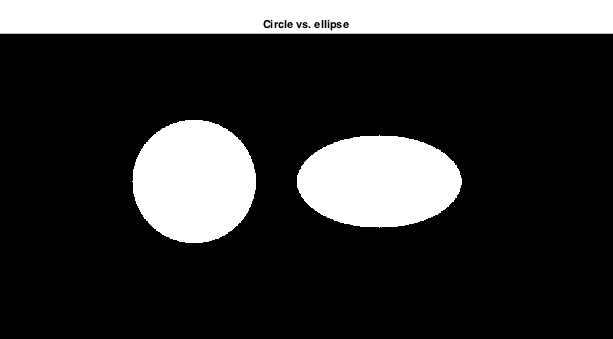
\includegraphics[width=0.6\textwidth]{billeder/software/circleellipse.png}
	\caption{Cirkel sammenlignet med ellipse}
	\label{fig:circleelip}
\end{figure}

Indekset for det objekt med mindst forskel i radius og indekset for det objekt med den mindste excentricitet gemmes i variabler. 
Til sidst i segmenteringen af den langerhanske ø kontrolleres det om radius forskellen og excentricitet ligger under nogle fast definerede grænseværdier. Værdierne er fundet ved at analysere en række billeder og deres objekters radius og excentricitet. Radius og excentriciteten bliver gemt i logfilen, så de kan analyseres for senere at justere grænseværdierne. Hvis objektets værdier er under disse grænseværdier er en ø detekteret. Når en ø er detekteret illustreres det med en grøn ring på GUI.

For at løse udfordringen med, at den samme ø vil optræde på det næste billede, er der implementeret et smalt detekteringsvindue (100 pixels bredt). Opløsningen på billederne er 800*600 pixels. Når øen er detekteret inden for dette område bliver variablen isletDetected sat til true. Denne variabel anvendes til styring af ventilen. 
 
Figur \ref{fig:segmented} viser slutresultatet af segmenteringen, hvor masken kun indeholder den langerhanske ø fra det oprindelige billede. 


\begin{figure}[H]
	\centering
	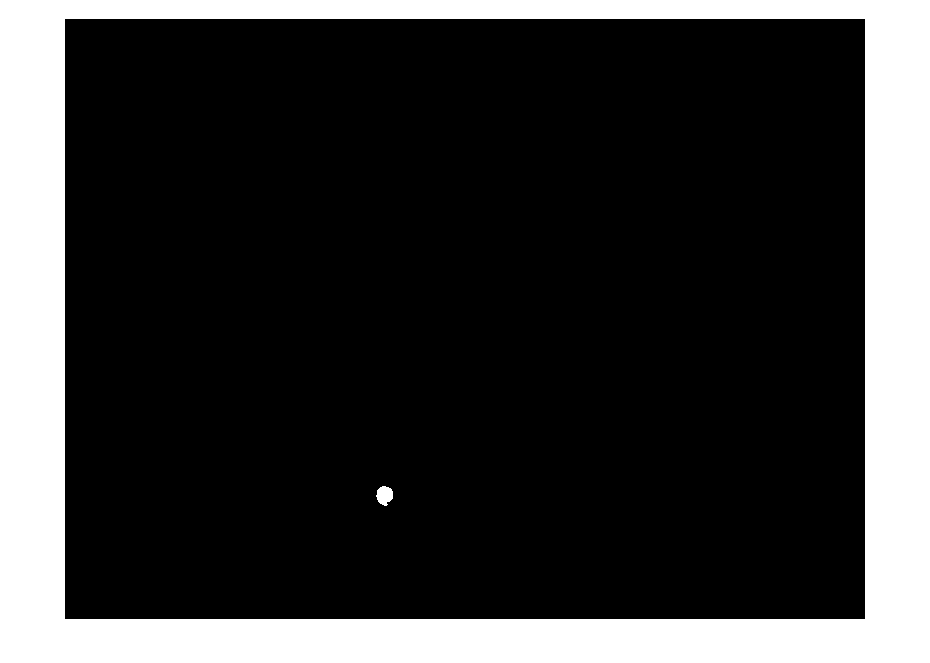
\includegraphics[width=0.6\textwidth]{billeder/software/segmented.png}
	\caption{Slutresultat af segmentering}
	\label{fig:segmented}
\end{figure}

I figur \ref{fig:finalimage} er det oprindelige billede vist, med markering af den detekterede ø.


\begin{figure}[H]
	\centering
	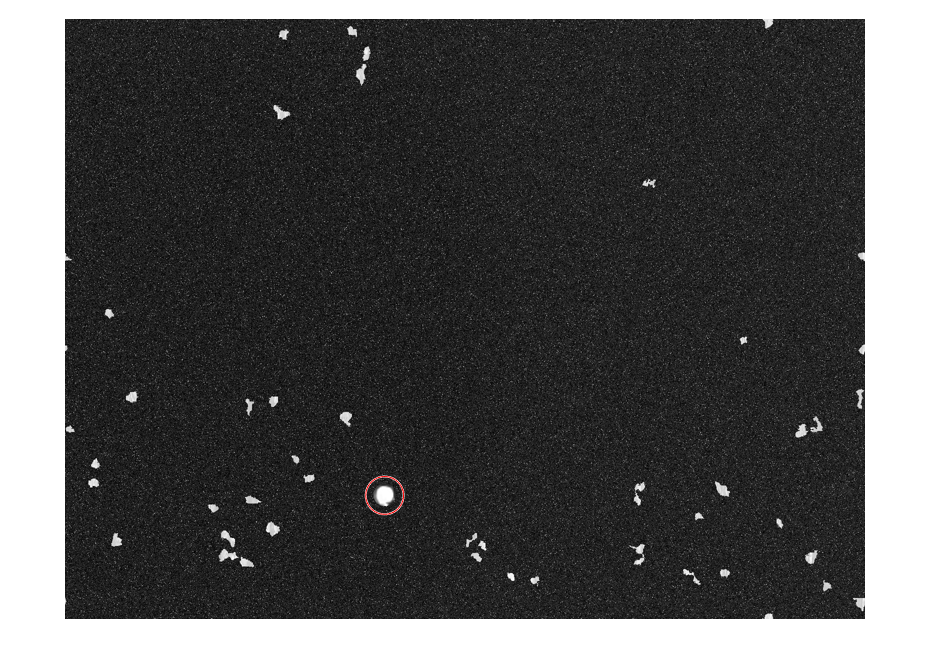
\includegraphics[width=0.6\textwidth]{billeder/software/finalimage.png}
	\caption{Oprindelige billede med detekteret ø}
	\label{fig:finalimage}
\end{figure}

\newpage
\textbf{Test af billedprocessering}

Udfordringen med billedprocesseringen er, at hastigheden ikke må være for langsom i forhold til frameraten for kameraet. Da et nyt billede indlæses hvert 0,1 sekund skal billedprocesseringen dermed være hurtigere end dette for at følge med. Til test af dette er Matlab funktionen tic/toc anvendt, som kan måle hvor langt tid billedprocessingen tager om at eksekvere. I figur \ref{fig:dataprocess} viser grafen hvor lang tid det har taget, at behandle de enkelte billeder. Den røde streg viser den gennemsnitlige tid for processeringen. For den nuværende implementering tager billedeprocessingen 0,0104 sekund pr. billede, hvilket er indenfor grænsen på 0,1 sekund. Tiden vil variere alt efter tilgængelig processorkraft og om der skal udføres andre opgaver, eksempelvis opdatere figurer på GUI. 

\begin{figure}[H]
	\centering
	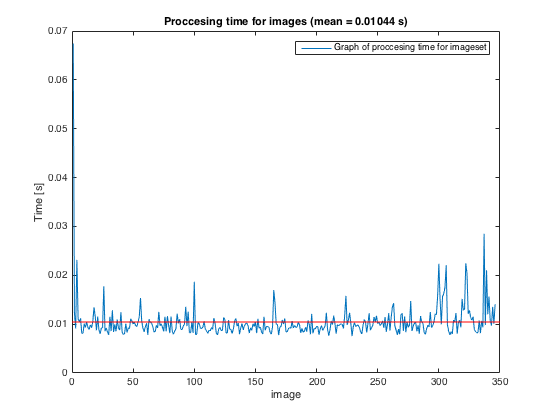
\includegraphics[width=0.6\textwidth]{billeder/software/dataprocessing_2.png}
	\caption{Test af tidsforbrug for billedeprocessering}
	\label{fig:dataprocess}
\end{figure}